\documentclass[12pt]{article}
\usepackage{geometry}
\geometry{margin=0.75in}
\usepackage{Style-Thesis-Report}
\renewcommand{\baselinestretch}{1}

\begin{document} 

	% Title
	\begin{center}
		\Large
		\textbf{Analyzing Regression Models on Symptoms Search Trend for COVID-19 Hospitalization Prediction }
		\vspace{0.5cm}
		
		\large
		Group 39 : Yuqi Liu, Anthony Ma, Chenxuan Zhou
		
		\today
	\end{center}
	
    % Abstract
    \hrule
	\begin{abstract} 
    The Coronavirus disease (COVID-19) is a highly infectious disease that has impacted and continues to impair the lives of people across the world. A plethora of approaches have been considered for analysis on the level of a pandemic outbreak. In particular, Google search trends can be used as an indicator of the daily thoughts and questioning of people that may reflect their health conditions. We, therefore, propose the utilization of Google Search Trends for the weekly symptom search trend data across regions in the US to predict the hospitalization cases. The primary objective of this project is to demonstrate K-Nearest-Neighbor Regression and Decision Tree Regression based on the symptom search trend dataset, with a comparison to weekly population mobility data. After comparing all models, we finally choose the one using the search trend dataset, split by time, and applied decision tree learning to be the best prediction strategy for this research.
	
	\end{abstract}
    \hrule

\section{Introduction}\label{sec:introduction}

Since the pandemic declaration by WHO in March, 2020, COVID-19 have remained the center of attention around the globe. Since the early stage of the pandemic, numerous efforts have been taken to predict the intensity of its spread. Among these works, the correlation between information-seeking behaviour \cite{mangono2020pace} and the COVID-19 outbreak can be explored for further use in the prediction of hospitalization cases.

\subsection{Search Trend Approach}
The study of Mangono \textit{et al.} noticed “substantial changes in coronavirus information-seeking at the national level, particularly in March 2020” due the COIVD-19\cite{mangono2020pace}. The result suggest a relation between search trend and COVID-19 event trends, which inspires us to turn our attention specifically to symptom search trends; we hypothesize that a machine learning model trained on symptom search trends and their hospitalization case numbers counterpart would achieve favorable performance.

\subsection{Social Distancing and Mobility}
The recommendation of Center for Disease Control and Prevention for “6 feet of distance”\cite{cdc} and the study by Parino \textit{et al.} \cite{parino2020modelling} using social distancing information to predict epidemic propagation both demonstrate that decreased mobility slows the spread of COVID-19. We therefore consider a mobility-based model as an adequate baseline model for our hospitalization case number prediction task.

\section{Materials and Methods}

\subsection{Datasets}

\subsubsection{Search Trend Dataset}
The first dataset, COVID-19 Search Trends symptoms dataset\cite{ds1}, contains symptoms search trends across different states in the US across different weeks from March to September, 2020. Symptoms and samples with more than 50\% empty entries were removed, leaving 27 out of the original 100 symptoms. The vacancy was filled with 0, with the assumption that the entries were 0 because of low search counts. Furthermore, we noticed a regional normalization in the data with non-uniform normalization factor. To offset such effect and render the data to be comparable across regions, each entry was updated as the percentage from mean within both its symptom and its region.

\subsubsection{Hospitalization Dataset}
The second dataset\cite{ds2} contains the daily number of new patients in the hospital daily over different regions. The data was aggregated into weekly data by averaging over each 7-day period. A merge by region and date was performed with the first dataset for the symptom search trend training and testing data.
 
 
\subsubsection{Mobility Dataset}
The third dataset, the Community Mobility Report\cite{ds3}, contains the percentage change of population mobility in public places in the US. The dataset was aggregated into weekly data and merged with the hospitalization dataset for the mobility training and testing data.

\subsection{Hyperparameter Selection}
For each KNN model the number of neighbours (k) was selected. The favored k is the value at which the decrease in loss begins to diminish; such a choice not only grants low loss but also ensures a small k which infers low computation complexity.

For each Decision Tree model the maximum tree depth (d) was selected. The favored d is the value at which the loss is the smallest. The random nature of Decision Tree training poses a challenge towards selecting the most optimal hyperparameter, but the produced by the selected models are sufficient for model comparison purposes.

\subsection{Train-Test Split by Region}
The preprocessed search trend dataset consists of data from twelve states in the United States of America. Therefore, a logical way of train-test split is separating the samples based on their region name. In consideration of the differences across regions, a 5-fold cross-validation was performed. The samples were split into 5 groups based on their $region\_name$ attribute. KNN and decision tree models were then cross-validated, the hyperparameters were selected, and the validation losses of the favored models were reported.

\subsection{Train-Test Split by Time}
Another logical method is splitting by date. A 80-20 train-test split was performed with data from first 24 weeks were taken as the training set and the rest as the validation set. KNN and decision tree models were simply trained and validated, hperparameters were selected, and validation losses were reported.


\subsection{Population Mobility in Public Places Report}
Using the mobility samples, KNN model was cross-validated in a split-by-time fashion, number of neighbours was selected, and the 5-fold cross-validation loss was reported.


\section{Results}

\subsection{Visualization of Symptom Search Trends}
\subsubsection{All symptoms across time}
The overall trend of symptom searches over time in the whole US was visualized as a heatmap to demonstrate variability and popularity of each symptom across time (Fig 4, Appendix 1). Several symptoms show high variability in popularity across time which may be due to the emergence of these symptoms as a result of COVID-19. 

\subsubsection{Specific symptom across region and time}
A few symptoms with high variability were selected and heatmaps were plotted to demonstrate their popularity across different regions throughout the weeks (Fig 5, Appendix 1).


\subsection{Visualization in Lower Dimensions}
\subsubsection{PCA}
The PCA dimension reduction tequnique was applied to produce a visualization of data in 2D. Additionally, the cumulative explained variances were examined over different number of PCA components. 5-component PCA was selected as it retains high variance while reduces dimensionality.

\begin{figure}[!htb]
    \centering
    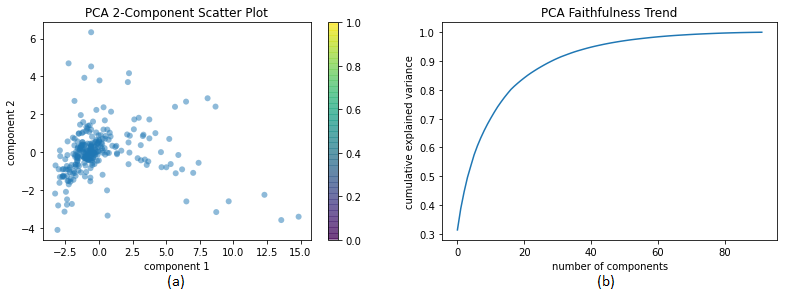
\includegraphics[scale=0.8]{pca}
    \caption{(a) PCA 2D Scatter Plot (b) Cumulative explained variance of PCA over different numbers of components}
\end{figure}


\subsubsection{K-Means}
To visualize the faithfulness of the PCA compression, K-Mean models were trained and graphed. The 2D cluster geometries obtained for the preprocessed data and the PCA data were not consistent; however, they can both infer 5 possible cluster groups from our dataset.

\begin{figure}[!htb]
    \centering
    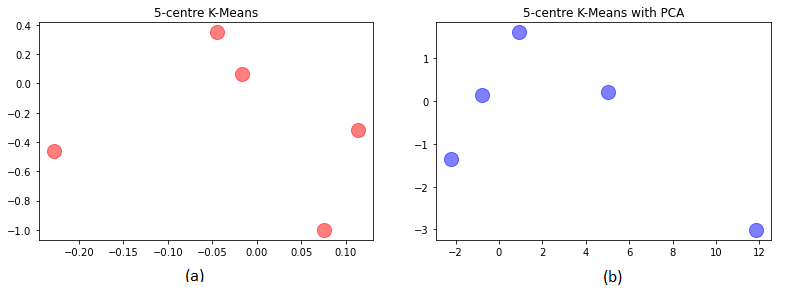
\includegraphics[scale=0.8]{k_means_comparison}
    \caption{K-Means clusters for (a) preprocessed data and (b) PCA data}
\end{figure}

\subsection{Model Training and Selection}
The hyperparameter (Table 1) and loss (Fig 3a) of each model were reported and their losses compared. The time-based-splitting approached resulted in the lowest loss, and overall the Decision Tree models performed better than KNN models. 
Additionally, feature selection was explored and the validation losses of the models reported (Fig 3b,3c).
\begin{table}[!htb]
\centering
\resizebox{\columnwidth}{!}{
\begin{tabular}{|l|l|l|l|l|l|l|l|l|}
    \hline
    & region KNN & region Decision Tree & time KNN & time Decision Tree & PCA KNN & PCA Decision Tree & PCA Linear Regression & mobility KNN \\
    \hline
    hyperparameter (k or d) & 15    & 4     & 46    & 8     & 23    & 6     & -     & 15  \\
    \hline
    validation loss (MSE)   & 5077  & 5906  & 1828  & 856   & 2553  & 4098  & 2332  & 2478 \\
    \hline
\end{tabular}
}
\caption{\label{tab:table-name} Selected hyperparameters and validation losses for all models.}
\end{table}

\begin{figure}[!htb]
    \centering
    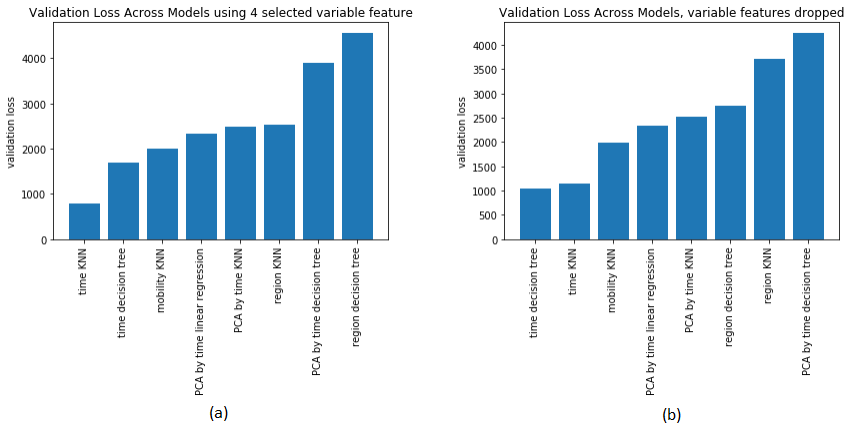
\includegraphics[scale=0.75]{feature_selection}
    \caption{Validation loss of different models using (a) all preprocessed data, (b) only selected symptoms, namely Viral pneumonia, Laryngitis, Anosmia, and Aphonia, and (c) all symptoms excluding the selected symptoms}
\end{figure}

\section{Discussion}

\subsection{KNN and Decision Tree Comparison}
In general, Decision Tree models resulted in low validation loss. We reason that, firstly, KNN suffers from the curse of dimensionality due to over 20 symptoms as features. Second, KNN has very limited capability of dealing with missing values, whereas Decision Tree models are not so much affected by missing values. Last, the regional normalization of the raw dataset, even after our demeaning processing, affects the performance of our split by region model; Decision Tree is less sensitive to such bias of input.

\subsection{Sample Set Comparison}
Among all the search trend models, only the 5-component PCA KNN and the split-by-region KNN achieve a worse performance than the mobility KNN, which is considered a baseline for comparison. Therefore, we recommend the symptoms search trend dataset as a predictor for COVID-19 hospitalization, especially with train-test split by time.

\subsection{Symptom Search Trends and Mobility Comparison}
The the KNN model trained on the split-by-time symptom search trends resulted in less loss than that of the mobility trends, which affirms the symptom search trends as an adequate predictor for hospitalization case numbers. We propose that the correlation levels of the datasets to the target datasets might be due to time delay. According to the World Health Organization, COVID-19 symptoms usually appear around 7 to 14 days after contraction. We postulate that a rise in population mobility might cause a rise in hospitalized patients in a time range longer than that of what symptoms search trend would, causing search trends to correlate with hospitalization data more than the population mobility trend when trained in a split-by-time method.

\subsection{Feature-Selection Comparison}
The selection and exclusion of highly variable symptoms observed in the heatmap have not resulted in significant increase in performance across models (Fig 3). Therefore, noise-reduction technique still requires further exploration.


\section{Conclusion}
From the above comparisons, we find that the best combination between datasets, splitting method, and learning approach for the search trend dataset is test-train split by time using Decision Tree in our settings. However, this does not make the model we chose the "absolute best one". As we discussed above, the fact that splitting by time is better than by region and the decision tree performs slightly better than KNN is due to our regional-biased dataset.
Hence, in future research, we still need to carefully analyze our dataset using different approaches to select the best model and strategy.



\bibliographystyle{IEEEtran} 
\bibliography{references}


\newpage
\large
\textbf{Appendix 1 : Visualization of Symptoms}
\begin{figure}[!htb]
    \centering
    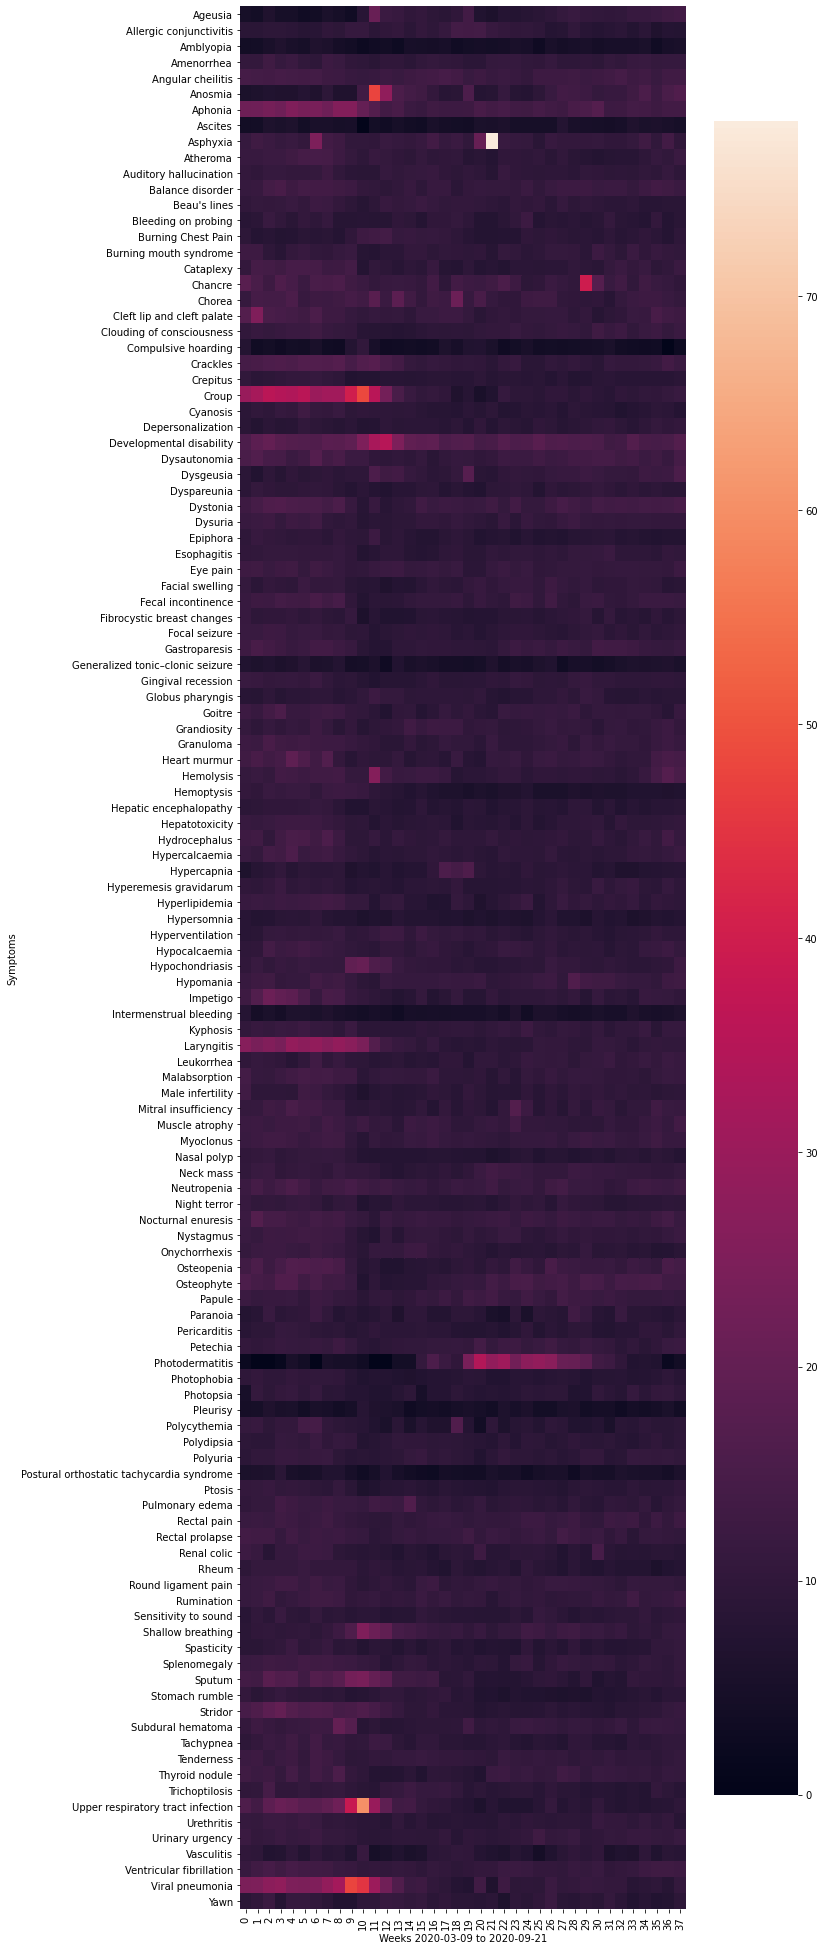
\includegraphics[scale=0.3]{symptoms}
    \caption{All symptoms over time.}
\end{figure}

\begin{figure}[!htb]
    \centering
    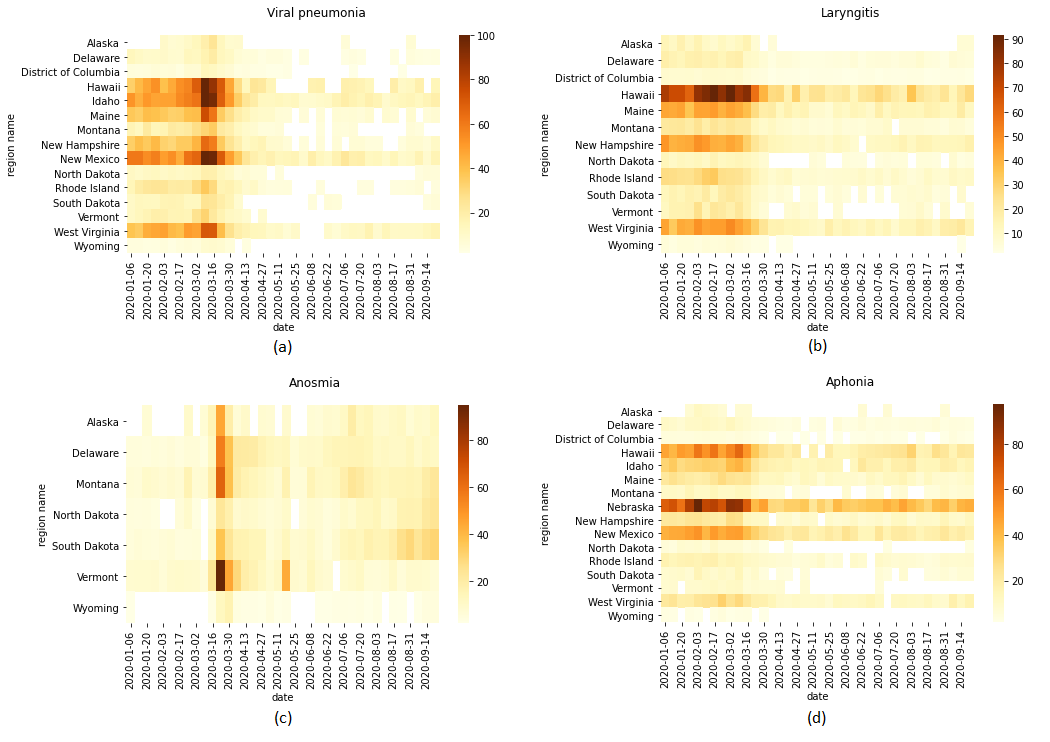
\includegraphics[scale=0.85]{high_variability_symptoms}
    \caption{High variability symptoms over region over time.}
\end{figure}



\end{document}